\begin{figure}[h!]
    \centering
    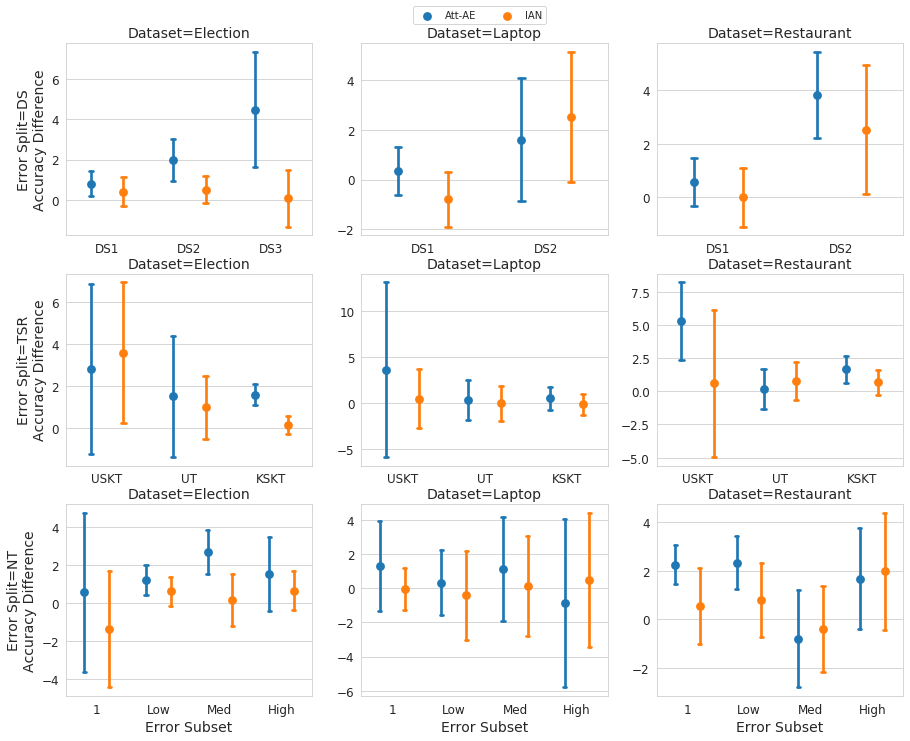
\includegraphics[scale=0.32]{images/augmentation/methods_performance/Position_Encoding/position_split_difference_validation_results.png}
    \caption{Columns represent different datasets, rows different error splits. Each plot represents the differences between the position and baseline models for the Accuracy metric on the given error subset. Validation split results.}
    \label{fig:aug_position_split_difference_validation_results}
\end{figure}

\begin{figure}[h!]
    \centering
    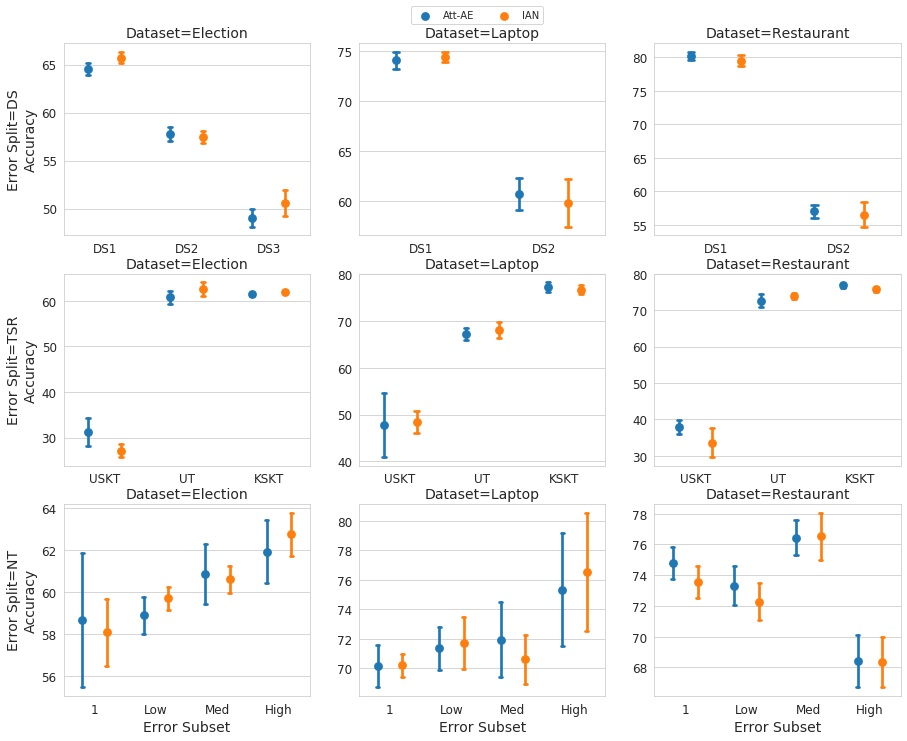
\includegraphics[scale=0.32]{images/augmentation/methods_performance/Position_Encoding/position_split_overall_validation_results.png}
    \caption{Columns represent different datasets, rows different error splits. Each plot represents the Accuracy metric for the position models on the given error subset. Validation split results.}
    \label{fig:aug_position_split_overall_validation_results}
\end{figure}

\begin{figure}[h!]
    \centering
    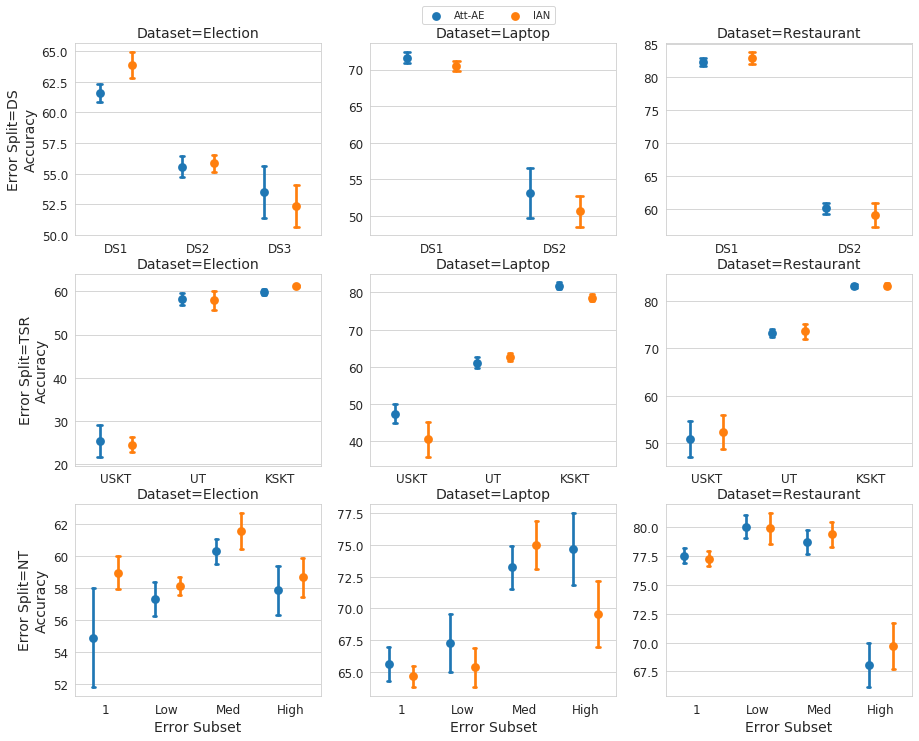
\includegraphics[scale=0.32]{images/augmentation/methods_performance/Position_Encoding/position_split_overall_test_results.png}
    \caption{Columns represent different datasets, rows different error splits. Each plot represents the Accuracy metric for the position models on the given error subset. Test split results.}
    \label{fig:aug_position_split_overall_test_results}
\end{figure}